\documentclass[paper = a4]{scrartcl}

\usepackage[T1]{fontenc}
\usepackage[utf8]{inputenc}
\usepackage[ngerman]{babel}
\usepackage[autostyle = true, german = quotes]{csquotes} % Anführungszeichen

\usepackage{amsmath}
\usepackage{graphicx}

\begin{document}

\subject{Praktikum Multicore"=Programmierung}
\title{Protokoll zu Projekt~6: Mehrgittermethoden}
\author{Florian Klemme \and Manuel Leßmann}
\maketitle

\section{Jakobi- und Gauß-Seidel-Verfahren}

%\begin{quote} a) Programmieren Sie eine serielle Version des Jakobi"=Verfahrens. Gegeben sei dazu [\dots] \(f(x, y) = 32(x(1 - x) + y(1 - y))\). Beachten Sie dabei auch die Randbedingungen [\(u(x, y) = 0 \quad \forall (x, y) \in \Gamma\)]. Verwenden Sie zur Überprüfung Ihres Programms auf Korrektheit die analytische Lösung \(u(x, y) = 16x(1 - x)y(1 - y) \quad \forall (x, y) \in \Omega\). \end{quote}

%\begin{quote} b) Implementieren Sie ebenfalls eine serielle Version des Gauß"=Seidel"=Verfahrens. Vergleichen Sie die gewonnenen Ergebnisse mit den Ergebnissen des Jakobi"=Verfahrens. Was fällt beim Vergleich der Iterationsschrittzahlen sowie der Laufzeiten beider Verfahren über verschiedenen Verfeinerungen (\(h = \frac{1}{2^l} \text{ mit } l = 1, 2, \dots, 6, \dots\)) auf? \end{quote}

%\begin{quote} c) Messen Sie mit Hilfe der in a) angegebenen analytischen Lösung für beide Verfahren den maximalen Approximationsfehler mit Hilfe der euklidischen Norm in jedem Iterationsschritt und für ein gewähltes h und stellen Sie diesen graphisch dar. \end{quote}

Bei der Darstellung des maximalen Approximationsfehlers in Abbildung~\ref{fig:fehler} ist die unterschiedlich schnelle Konvergenz des Jakobi"= und des Gauß"=Seidel"=Verfahrens deutlich erkennbar. Beide Verfahren näheren sich logarithmisch der analytisch Lösung an.

\begin{figure}
    \centering
    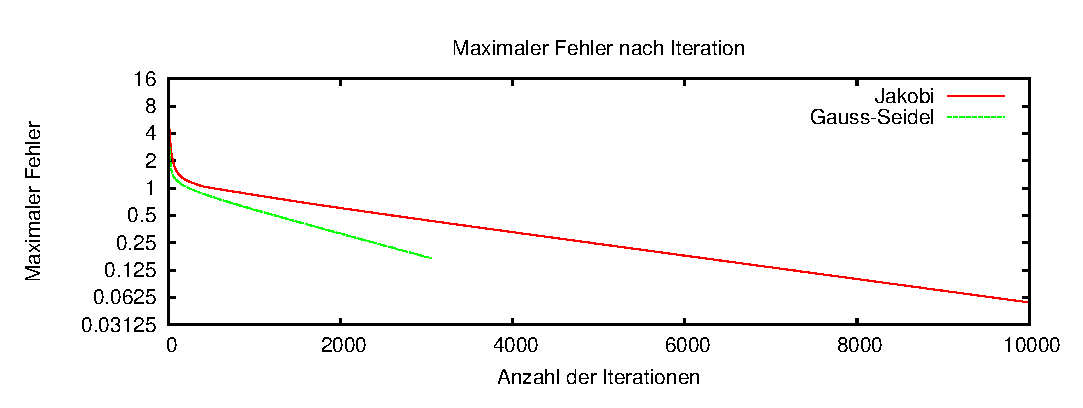
\includegraphics[width=\textwidth]{fehler}
    \caption{Maximaler Approximationsfehlers nach jedem Iterationsschritt.}
    \label{fig:fehler}
\end{figure}

%\begin{quote} d) Da hier innerhalb eines einzelnen Iterationsschritts keine Datenabhängigkeiten zu finden sind, lässt sich das Jakobi"=Verfahren durch einfaches Aufteilen der Berechnungen auf verscheidene Prozessoren und Kommunizieren eventueller Überlappungen parallelisieren. Entwerfen Sie eine parallele Version des Verfahrens (wahlweise mit OpenMP oder Cuda/OpenCL) und verifizieren Sie Ihre Ergebnisse gegenüber der seriellen Variante. \end{quote}

%\begin{quote} e) Im Gegensatz zum Jakobi"=Verfahren zeigt das Gauß"=Seidel"=Verfahren Datenabhängigkeiten innerhalb der einzelnen Iterationsschritte. Daher eignet sich eine naive Herangehensweise nicht, um dieses Verfahren ausreichend zu parallelisieren. Ihre Aufgabe ist es, eine sinnvolle Methodik zu entwickeln, mit welcher sich dieses Verfahren parallelisieren lässt. \end{quote}

Die Datenabhängigkeiten im Gauß"=Seidel"=Verfahren erschweren die Parallelisierung. Zumindest alle Felder auf der Diagonalen des Ergebnisvektors lassen sich aber parallel verarbeiten. Von hier aus kann diese Diagonale dann Feld für Feld über den Ergebnisvektor verschoben werden, sodass bis zu \(\frac{1}{h} - 1\) Threads gleichzeitig arbeiten können.

%\begin{figure}
%    \centering
%    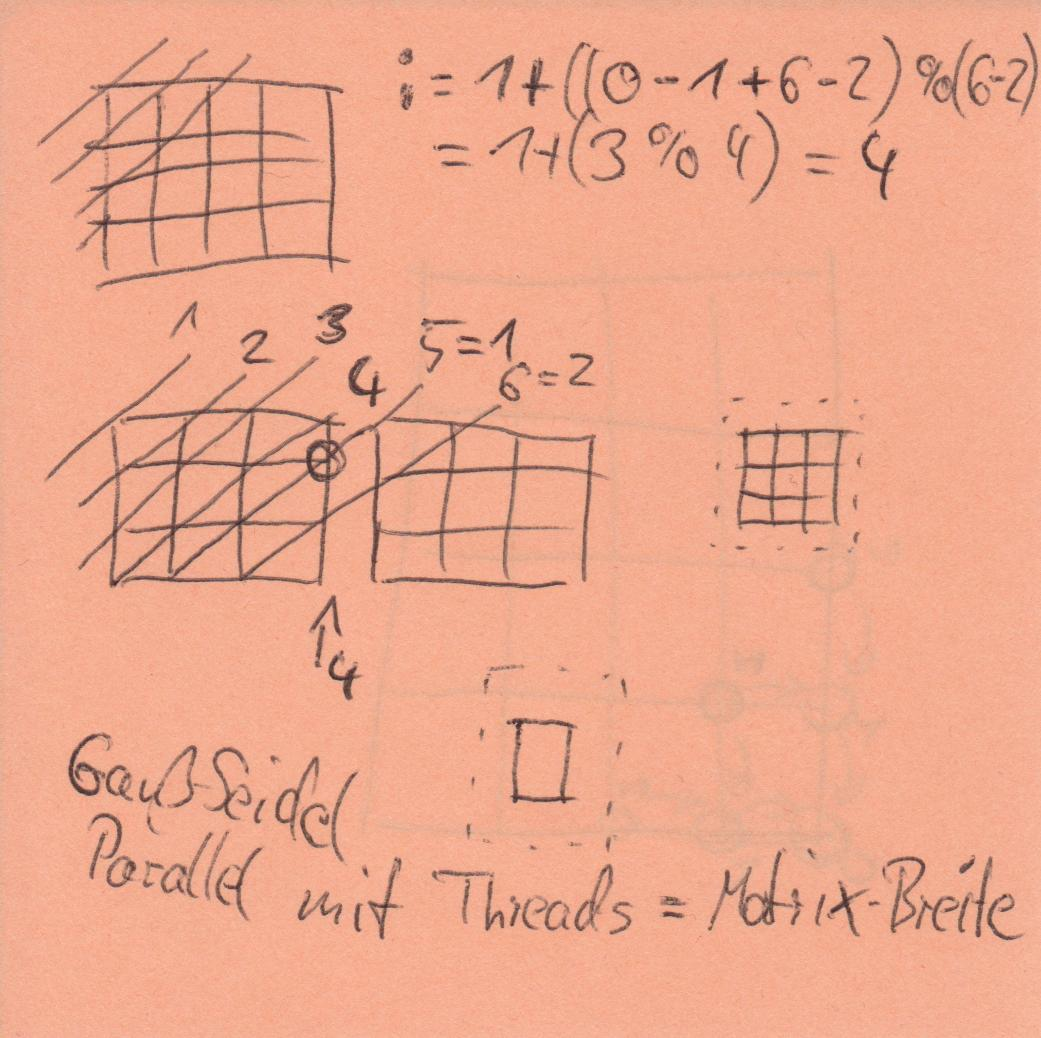
\includegraphics[width=0.5\textwidth]{gaussseidelskizze}
%    \caption{Skizze zum Entwurfsgedanken zu Gauß"=Seidel, parallel.}
%    \label{fig:gaussseidelskizze}
%\end{figure}

Abbildung~\ref{fig:gaussseideldreiecke} skizziert eine Verbesserung der Threadauslastung, bei der voneinander abhängige Felder in Gruppen zusammengefasst werden, die wiederum unabhängig voneinander bearbeitet werden können. Dies verringert den Synchronisierungs"=Overhead beim Wechsel zum nächsten Datenfeld.

\begin{figure}
    \centering
    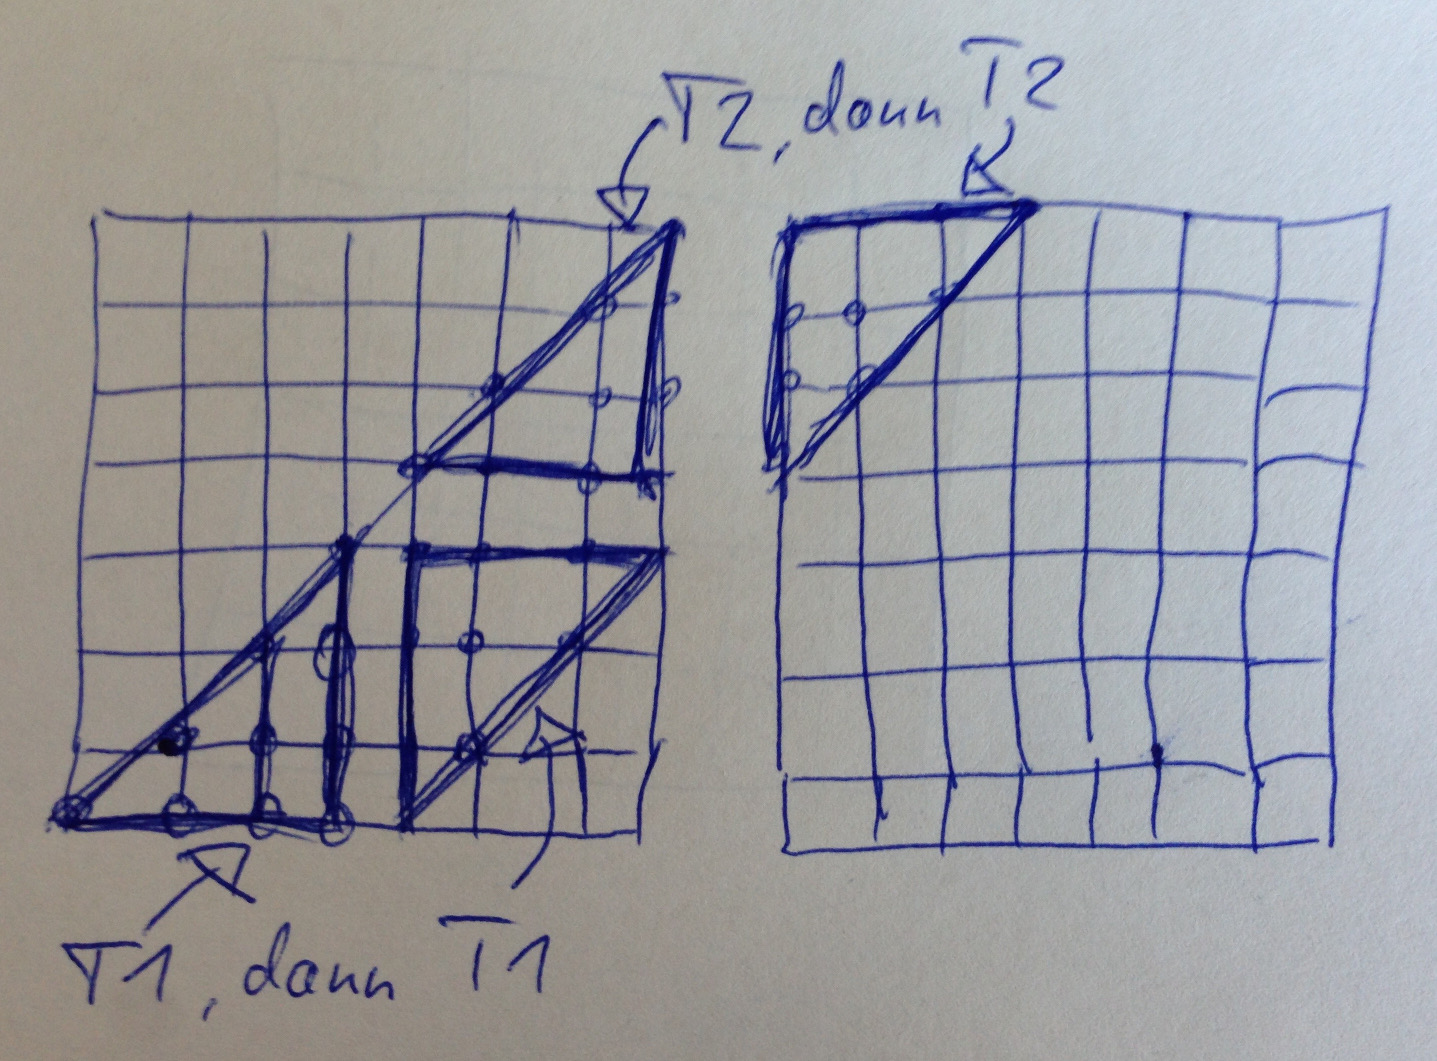
\includegraphics[width=0.5\textwidth]{gaussseideldreiecke}
    \caption{Verbesserung der Threadauslastung durch Bildung von Gruppen. Alle diagonal zueinander stehenden Dreiecke mit der gleichen Nummer könnne parallel verarbeitet werden.}
    \label{fig:gaussseideldreiecke}
\end{figure}

%\begin{quote} f) Ermitteln Sie den Speedup für verschiedene Problemgrößen für beide Verfahren (\(h = \frac{1}{2^l} \text{ mit } l = 1, 2, \dots, 6, \dots\)). Beurteilen Sie damit auch die Qualität ihrer Parallelisierungen. \end{quote}

\section{Mehrgitter-Verfahren}

\emph{Warum ist es aus Sicht der Numerik nicht sinnvoll sofort auf einem groben Gitter zu beginnen, sondern zunächst einige Schritte auf einem feinen Gitter durchzuführen?}

Ein grobes Gitter führt zwangsläufig zu Undersampling. Gerade bei hochfrequenten Funktionen entstehen dadurch schwerwiegende Aliasingeffekte, die sich auch durch die Ausführung von Gauß"=Seidel nicht verringern lassen, da die Informationen schlicht im Startvektor nicht enthalten sind. Deshalb sollte man zunächst auf feineren Gittern iterieren. Dadurch erstellt man einen Startvektor, der zwar dieselbe Feinheit hat, jedoch auch Informationen aus den hochfrequenten Teilen der Funktionen beinhaltet. Dieses Verfahren führt zur Glättung des Fehlers, der zwangsläufig durch Aliasing entsteht.

Die Tabellen~\ref{tab:b} bis~\ref{tab:f} zeigen verschiedene Benchmark"=Ergebnisse und vergleichen Algorithmen und Parameter"=Konfigurationen miteinander.
% TODO: Abschließender Satz zu "welches der vorgestellten Verfahren Sie für geeigneter halten um Gleichungssysteme großer Dimension zu lösen".

%\subsection*{b)}
\begin{table}
    \centering
    \begin{tabular}{|r|r|r|r|r|} \hline
    & & Laufzeit in & \multicolumn{2}{c|}{Approx. Fehler} \\
    z1 & z2 & Sekunden & Mittel & Maximum \\ \hline \hline
    4  & 4  & 0,0599   & 0,0324 & 0,0880  \\
    4  & 8  & 0,0634   & 0,0321 & 0,0877  \\
    4  & 16 & 0,0715   & 0,0314 & 0,0871  \\
    4  & 32 & 0,0876   & 0,0305 & 0,0859  \\ \hline
    8  & 4  & 0,0634   & 0,0323 & 0,0877  \\
    8  & 8  & 0,0674   & 0,0320 & 0,0874  \\
    8  & 16 & 0,0755   & 0,0313 & 0,0868  \\
    8  & 32 & 0,0946   & 0,0304 & 0,0856  \\ \hline
    16 & 4  & 0,0714   & 0,0321 & 0,0871  \\
    16 & 8  & 0,0755   & 0,0317 & 0,0868  \\
    16 & 16 & 0,0835   & 0,0311 & 0,0862  \\
    16 & 32 & 0,0997   & 0,0302 & 0,0850  \\ \hline
    32 & 4  & 0,0876   & 0,0317 & 0,0859  \\
    32 & 8  & 0,0916   & 0,0313 & 0,0857  \\
    32 & 16 & 0,0997   & 0,0307 & 0,0851  \\
    32 & 32 & 0,1159   & 0,0298 & 0,0839  \\ \hline
    \end{tabular}
    \caption{Mehrgitter"=Verfahren: Offensichtlich hat \(z2\) einen deutlich größeren Einfluss auf den Fehler als \(z1\). Konfiguration: \(n=256, h_{max}=h*4, alpha=1\).}
    \label{tab:b}
\end{table}

%\subsection*{c)}
\begin{table}
    \centering
    \begin{tabular}{|r|r|r|r|} \hline
    & & \multicolumn{2}{c|}{Approx. Fehler} \\
    n    & alpha & Mittel & Maximum \\ \hline \hline
    256  & 1     & 0,0771 & 0,1962  \\
    256  & 2     & 0,0771 & 0,1962  \\
    512  & 1     & 0,0431 & 0,1052  \\
    512  & 2     & 0,0431 & 0,1053  \\
    1024 & 1     & 0,0321 & 0,0853  \\
    1024 & 2     & 0,0222 & 0,0548  \\
    2048 & 1     & 0,2341 & 0,5783  \\
    2048 & 2     & 0,0111 & 0,0289  \\ \hline
    \end{tabular}
    \caption{Ein höherer Alpha"=Wert führt besonders bei großer Gitterfeinheit und wenig Iterationen zu deutlich geringeren Fehlern. Konfiguration: \(z1=z2=4, h_{max} = 16*h\).}
    \label{tab:c}
\end{table}

%\subsection*{e)}
\begin{table}
    \centering
    \begin{tabular}{|r|r|r|r|r|} \hline
    & \multicolumn{2}{c|}{Laufzeit in Sekunden} & & \\
    n    & Seq. Zeit & Par. Zeit & Speedup & Effizienz \\ \hline \hline
    16   & 0,0004    & 0,0072    & 0,0567  & 0,0142    \\
    32   & 0,0016    & 0,0139    & 0,1124  & 0,0281    \\
    64   & 0,0067    & 0,0379    & 0,1765  & 0,0441    \\
    128  & 0,0350    & 0,1045    & 0,3352  & 0,0838    \\
    256  & 0,1422    & 0,1522    & 0,9338  & 0,2334    \\
    512  & 0,5698    & 0,3205    & 1,7780  & 0,4445    \\
    1024 & 2,3061    & 0,9857    & 2,3397  & 0,5849    \\
    2048 & 9,2382    & 3,6254    & 2,5482  & 0,6371    \\ \hline
    \end{tabular}
    \caption{Welche Ergebnisse sind das hier? Konfiguration: \(alpha=2, z1=z2=32, h_{max} = 8*h\).}
    \label{tab:e}
\end{table}

%\subsection*{f)}
\begin{table}
    \centering
    \begin{tabular}{|l|r|r|r|r|r|r|} \hline
    & \multicolumn{2}{c|}{Laufzeit in Sekunden} & & & \multicolumn{2}{c|}{Approx. Fehler} \\
    Algorithmus & Seq. Zeit & Par. Zeit & Speedup & Effizienz & Mittel   & Maximum \\ \hline \hline
    Jakobi      & 33,9062   & 19,2902   & 1,7577  & 0,4394    & 0,4443   & 0,9990  \\
    Gauß-Seidel & 52,3843   & 19,5082   & 2,6853  & 0,6713    & 0,4436   & 0,9981  \\
    Mehrgitter  & 2,5800    & 1,3330    & 1,9354  & 0,4838    & 0,0111   & 0,0289  \\ \hline
    \end{tabular}
    \caption{Bei einer Beschränkung auf 1000~Iterationen kommt die Stärke des Mehrgitter"=Verfahrens deutlich zum Vorschein. Konfiguration: \(n=2048, alpha=2, z1=z2=4, h_{max}=16*h\).}
    \label{tab:f}
\end{table}

\end{document}
